\documentclass[11pt, compress]{beamer}
\usepackage{amsmath}
\usetheme{Boadilla}
\usefonttheme[onlymath]{serif}
%get rid of navigation:
\setbeamertemplate{navigation symbols}{}


 %%%% Start PreTeXt generated preamble: %%%%% 

%% Some aspects of the preamble are conditional,
%% the LaTeX engine is one such determinant
\usepackage{ifthen}
\newcommand{\tabularfont}{}
\usepackage[xparse, raster]{tcolorbox}
\tcbset{colback=white, colframe=white}
\NewTColorBox{image}{mmm}{boxrule=0.25pt, colframe=gray, left skip=#1\linewidth,width=#2\linewidth}
\RenewTColorBox{definition}{m}{colback=teal!30!white, colbacktitle=teal!30!white, coltitle=black, colframe=gray, boxrule=0.5pt, sharp corners=downhill, titlerule = 0.25pt, title={#1}}
\RenewTColorBox{theorem}{m}{colback=pink!30!white, colbacktitle=pink!30!white, coltitle=black, colframe=gray, boxrule=0.5pt, sharp corners=downhill, titlerule = 0.25pt, title={#1}}
\RenewTColorBox{proof}{}{boxrule=0.25pt, colframe=gray, colback=white, before upper={Proof:}, after upper={\qed}}
%% tcolorbox styles for sidebyside layout
\tcbset{ bwminimalstyle/.style={size=minimal, boxrule=-0.3pt, frame empty,
colback=white, colbacktitle=white, coltitle=black, opacityfill=0.0} }
\tcbset{ sbsstyle/.style={raster before skip=2.0ex, raster equal height=rows, raster force size=false} }
\tcbset{ sbspanelstyle/.style={bwminimalstyle} }
%% Enviroments for side-by-side and components
%% Necessary to use \NewTColorBox for boxes of the panels
%% "newfloat" environment to squash page-breaks within a single sidebyside
%% "xparse" environment for entire sidebyside
\NewDocumentEnvironment{sidebyside}{mmmm}
  {\begin{tcbraster}
    [sbsstyle,raster columns=#1,
    raster left skip=#2\linewidth,raster right skip=#3\linewidth,raster column skip=#4\linewidth]}
  {\end{tcbraster}}
%% "tcolorbox" environment for a panel of sidebyside
\NewTColorBox{sbspanel}{mO{top}}{sbspanelstyle,width=#1\linewidth,valign=#2}
\newcommand{\lt}{<}
\newcommand{\gt}{>}
\newcommand{\amp}{&}

%% Begin: Semantic Macros
%% To preserve meaning in a LaTeX file
%%
%% \mono macro for content of "c", "cd", "tag", etc elements
%% Also used automatically in other constructions
%% Simply an alias for \texttt
%% Always defined, even if there is no need, or if a specific tt font is not loaded
\newcommand{\mono}[1]{\texttt{#1}}
%%
%% Following semantic macros are only defined here if their
%% use is required only in this specific document
%%
%% Used for inline definitions of terms
\newcommand{\terminology}[1]{\textbf{#1}}
%% End: Semantic Macros

\renewcommand{\d}{\displaystyle}
\newcommand{\N}{\mathbb N}
\newcommand{\B}{\mathbf B}
\newcommand{\Z}{\mathbb Z}
\newcommand{\Q}{\mathbb Q}
\newcommand{\R}{\mathbb R}
\def\C{\mathbb C}
\def\U{\mathcal U}
\newcommand{\pow}{\mathcal P}
\newcommand{\inv}{^{-1}}
\newcommand{\st}{:}
\renewcommand{\iff}{\leftrightarrow}
\newcommand{\Iff}{\Leftrightarrow}
\newcommand{\imp}{\rightarrow}
\newcommand{\Imp}{\Rightarrow}
\newcommand{\isom}{\cong}

\renewcommand{\bar}{\overline}
\newcommand{\card}[1]{\left| #1 \right|}
\newcommand{\twoline}[2]{\begin{pmatrix}#1 \\ #2 \end{pmatrix}}

\newcommand{\vtx}[2]{node[fill,circle,inner sep=0pt, minimum size=4pt,label=#1:#2]{}}
\newcommand{\va}[1]{\vtx{above}{#1}}
\newcommand{\vb}[1]{\vtx{below}{#1}}
\newcommand{\vr}[1]{\vtx{right}{#1}}
\newcommand{\vl}[1]{\vtx{left}{#1}}
\renewcommand{\v}{\vtx{above}{}}

%% Graphics Preamble Entries
\usepackage{tikz, pgfplots}

\usetikzlibrary{positioning,matrix,arrows}

\usetikzlibrary{shapes,decorations,shadows,fadings,patterns}
\usetikzlibrary{decorations.markings}

\usepackage{skak} %for chessboards etc.

\def\circleA{(-.5,0) circle (1)}
\def\circleAlabel{(-1.5,.6) node[above]{$A$}}
\def\circleB{(.5,0) circle (1)}
\def\circleBlabel{(1.5,.6) node[above]{$B$}}
\def\circleC{(0,-1) circle (1)}
\def\circleClabel{(.5,-2) node[right]{$C$}}
\def\twosetbox{(-2,-1.4) rectangle (2,1.4)}
\def\threesetbox{(-2.5,-2.4) rectangle (2.5,1.4)}
\newcommand{\hexbox}[3]{
  \def\x{-cos{30}*\r*#1+cos{30}*#2*\r*2}
  \def\y{-\r*#1-sin{30}*\r*#1}
  \draw (\x,\y) +(90:\r) -- +(30:\r) -- +(-30:\r) -- +(-90:\r) -- +(-150:\r) -- +(150:\r) -- cycle;
  \draw (\x,\y) node{#3};
}

\tikzset{->-/.style={decoration={
  markings,
  mark=at position .5 with {\arrow{>}}},postaction={decorate}}}

  \newcommand{\onedot}{
    +(.5,.5) \v
  }
  \newcommand{\twodots}{
    +(.25,.25) \v +(.75,.75) \v
  }
  \newcommand{\threedots}{
  +(.25,.25) \v +(.5, .5) \v +(.75,.75) \v
  }
  \newcommand{\fourdots}{
    +(.25,.25) \v +(.25,.75) \v +(.75,.25) \v +(.75,.75) \v
  }
  \newcommand{\fivedots}{
    +(.5,.5) \v +(.25,.25) \v +(.25,.75) \v +(.75,.25) \v +(.75,.75) \v
  }
  \newcommand{\sixdots}{
    +(.25,.5) \v +(.75,.5) \v +(.25,.25) \v +(.25,.75) \v +(.75,.25) \v +(.75,.75) \v
  }
  \newcommand{\dominoborder}{
    \draw[thick, rounded corners] (0,0) rectangle (1,2);
    \draw[thin] (0,1) -- (1,1);
  }


%%%% End of PreTeXt generated preamble %%%%% 

\title{Combinatorial Proofs}
\subtitle{(Section 1.4)}
\author{}
\date[]{}

\begin{document}
\begin{frame}
\maketitle 
\end{frame}
 
\begin{frame}
\frametitle{Overview}
\tableofcontents 
\end{frame}
 

\section{Warm-up}
\begin{frame}
\frametitle{Investigate!}
 \begin{enumerate}
\item{} The Stanley Cup is decided in a best of 7 tournament between two teams. In how many ways can your team win? Let's answer this question two ways:\begin{enumerate}
\item{} How many of the 7 games does your team need to win? How many ways can this happen?


\item{} What if the tournament goes all 7 games? So you win the last game. How many ways can the first 6 games go down?


\item{} What if the tournament goes just 6 games? How many ways can this happen? What about 5 games? 4 games?


\item{} What are the two different ways to compute the number of ways your team can win? Write down an equation involving binomial coefficients (that is, \({n \choose k}\)'s). What pattern in Pascal's triangle is this an example of?

\end{enumerate}



\item{} Generalize. What if the rules changed and you played a best of \(9\) tournament (5 wins required)? What if you played an \(n\) game tournament with \(k\) wins required to be named champion?

\end{enumerate}

\end{frame}
 


\section{Patterns in Pascal's Triangle}
\begin{frame}
\frametitle{Patterns in Pascal's Triangle}
 Have a look again at Pascal's triangle. Forget for a moment where it comes from. Just look at it as a mathematical object. What do you notice?
 \begin{sidebyside}{1}{0.25}{0.25}{0}%
\begin{sbspanel}{0.5}%
\resizebox{\linewidth}{!}{%
        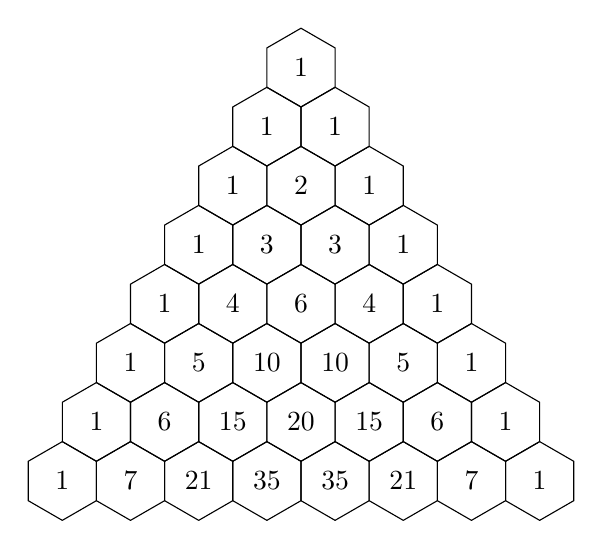
\begin{tikzpicture}
\def\r{.5}

% Pascal's triangle
%put row of 1's down left side:
  \foreach \row in {0,...,7} {
    \hexbox{\row}{0}{ 1}
  }
%fill in the rest of the triangle:
  \foreach \row in {1,...,7} {
    \pgfmathsetmacro{\entry}{1};
    \foreach \col in {1,...,\row} {
      % iterative formula : val = precval * (row-col+1)/col
      % (+ 0.5 to bypass rounding errors)
     \pgfmathtruncatemacro{\entry}{\entry*((\row-\col+1)/\col)+0.5}; \global\let\entry=\entry
      \ifnum \entry<100
	\hexbox{\row}{\col}{\entry}
      \else \ifnum \entry<1000
	\hexbox{\row}{\col}{\footnotesize \entry}
      \else \ifnum \entry<10000
	\hexbox{\row}{\col}{\footnotesize \entry}
	\else
	\hexbox{\row}{\col}{\scriptsize \entry}
	\fi
      \fi
      \fi
    }
  }
\end{tikzpicture}
}%
\end{sbspanel}%
\end{sidebyside}%
\end{frame}
 
\begin{frame}
\frametitle{A few patterns}
 \begin{enumerate}
\item{} The entries on the border of the triangle are all 1.


\item{} Any entry not on the border is the sum of the two entries above it.


\item{} The triangle is symmetric. In any row, entries on the left side are mirrored on the right side.


\item{} The sum of all entries on a given row is a power of 2. (You should check this!)

\end{enumerate}

\end{frame}
 
\begin{frame}
\frametitle{Binomial Identities}
 The previous observations can be rewritten:\begin{enumerate}
\item{} \({n \choose 0} = 1\) and \({n \choose n} = 1\).

\item{} \({n \choose k} = {n-1 \choose k-1} + {n-1 \choose k}\).

\item{} \({n \choose k} = {n \choose n-k}\).

\item{} \({n\choose 0} + {n \choose 1} + {n \choose 2} + \cdots + {n \choose n} = 2^n\).
\end{enumerate}

 
\pause \vfill 

Each of these is an example of a \terminology{binomial identity}: an identity (i.e., equation) involving binomial coefficients.
\end{frame}
 
\begin{frame}
\frametitle{}
\begin{example}[1.4.1]Give an algebraic proof for the binomial identity%
\begin{equation*}
{n \choose k} = {n-1\choose k-1} + {n-1 \choose k}\text{.}
\end{equation*}


\pause \vfill 

Starting with the right-hand side of the equation:%
\begin{align*}
{n-1 \choose k-1} + {n-1 \choose k} \amp = \frac{(n-1)!}{(n-k)!(k-1)!}+ \frac{(n-1)!}{(n-1-k)!\,k!}\\
\amp = \frac{(n-1)!k}{(n-k)!\,k!} + \frac{(n-1)!(n-k)}{(n-k)!\,k!}\\
\amp = \frac{(n-1)!(k+n-k)}{(n-k)!\,k!}\\
\amp = \frac{n!}{(n-k)!\, k!} = {n \choose k}\text{.}
\end{align*}


\pause \vfill 

Yuck!  Our goal is to find a better style of proof for these identities.
\end{example}
\end{frame}
 
\begin{frame}
\frametitle{}
\begin{example}[1.4.2]Explain why \({n \choose 0} = 1\) and \({n \choose n} = 1\).

\pause \vfill 

Hint: What does \(\binom{n}{0}\) tell you in terms of subsets?
\end{example}
\end{frame}
 
\begin{frame}
\frametitle{}
\begin{example}[1.4.3]Explain why \({n \choose k} = {n-1 \choose k-1} + {n-1 \choose k}\).

\pause \vfill 

Hint: what does \(\binom{n}{k}\) tell you in terms of bit-strings?
\end{example}
\end{frame}
 
\begin{frame}
\frametitle{}
\begin{example}[1.4.4]Prove the binomial identity \({n \choose k} = {n \choose n-k}\).

\pause \vfill 

Hint: what does \(\binom{n}{k}\) tell you in terms of pizza toppings?
\end{example}
\end{frame}
 
\begin{frame}
\frametitle{}
\begin{example}[1.4.5]Prove the binomial identity \({n\choose 0} + {n \choose 1} + {n\choose 2} + \cdots + {n \choose n} = 2^n\).

\pause \vfill 

Hint: Try subsets or pizzas!  What question about subsets is \(2^n\) the answer to?  Why is the answer to that question also the left-hand side?
\end{example}
\end{frame}
 


\section{More Proofs}
\begin{frame}
\frametitle{Combinatorial Proofs}
 The explanatory proofs given in the above examples are typically called \terminology{combinatorial proofs}. In general, to give a combinatorial proof for a binomial identity, say \(A = B\) you do the following:
 
\pause \vfill 

\begin{enumerate}
\item{} Find a counting problem you will be able to answer in two ways.


\item{} Explain why one answer to the counting problem is \(A\).


\item{} Explain why the other answer to the counting problem is \(B\).

\end{enumerate}

 
\pause \vfill 

Since both \(A\) and \(B\) are the answers to the same question, we must have \(A = B\).
\end{frame}
 
\begin{frame}
\frametitle{Finding Questions}
 How many 10-letter words use exactly four A's, three B's, two C's and one D?
 
\pause \vfill 

Prove:%
\begin{equation*}
{10 \choose 4}{6 \choose 3}{3 \choose 2}{1 \choose 1} = {10 \choose 1}{9 \choose 2}{7 \choose 3}{4 \choose 4}
\end{equation*}

\end{frame}
 
\begin{frame}
\frametitle{}
\begin{example}[1.4.6]Prove the identity%
\begin{equation*}
1 n + 2(n-1) + 3 (n-2) + \cdots + (n-1) 2 + n 1 = {n+2 \choose 3}\text{.}
\end{equation*}

\end{example}
\end{frame}
 
\begin{frame}
\frametitle{}
\begin{example}[1.4.7]Prove the binomial identity%
\begin{equation*}
{n \choose 0}^2 + {n \choose 1}^2 + {n \choose 2}^2 + \cdots + {n \choose n}^2 = {2n \choose n}\text{.}
\end{equation*}

\end{example}
\end{frame}
 

\end{document}
